La QKD (Quantum Key distribution), o Distribuzione Quantistica delle Chiavi, \`e una tecnologia di crittografia quantistica che permette la distribuzione di chiavi crittografiche con un livello di sicurezza inattacabile anche da computer quantistici. La QKD pu\`o essere suddivisa in due macro-classi DV-QKD e CV-QKD. Nella DV-QKD (Descrete Variable Quantum Key Distribution) le informazioni vengono trasmesse utilizzando stati quantici discreti, ad esempio la polarizzazione degli fotoni, che viene misurata attravarso apposite apparecchiature per ogni fotone; al contrario nella CV-QKD (Continous Variable Quantum Key Distribution) vengono misurate variabili continue delle onde elettromagnatiche come ad esempio la fase.

La sicurezza \'e garantita dai principi delle fisica quantistica che ci permettono di rilevare eventuali intercettazioni da parte di Eve (spia) nella trasmissione su canale quantistico tra Alice (mittente) e Bob (destinatario).

La rilevazione \`e dovuta al fatto che durante la misura da parte di Eve lo stato quantistico viene alterato facendo diminuire l'energia del segnale e introducendo del rumore, quindi dell'incertezza. All'atto pratico Eve intercetta lo stato coerente, rappresentato come in figura~\ref{fig:stato-coerente}, ne effettua una misura per poi ritrasmetterlo sul canale. Bob ricever\`a uno stato coerente con del rumore aggiunto e un minor numero di fotoni, ci\`o comporta che la gaussiana che lo rappresenta sar\`a caratterizzata da una varianza superiore a quella stimata e un valor medio pi\`u vicino allo zero. Per questo motivo, si effettuano numerosi run di trasmissione quantistica. In una fase preliminare si utilizza un certo numero di run per stimare i parametri di rumore del canale e, da essi, decidere se la trasmissione sta avvenendo in modo sicuro oppure no (si veda Sez.~\ref{subse:stima-parametri}). Nel caso in cui il controllo non vada a buon fine, la trasmissione  corrente viene abbortita perch\'e non \`e possibile garantire la sicurezza della chiave crittografica.

\section{CV-QKD con modulazione gaussiana}
Il protocollo di distribuzione quantistica di chiavi a variabili continue con modulazione gaussiana \`e un protocollo molto indicato per lo sviluppo e l'utilizzo su larga scala nel mondo reale data la sua affinit\`a con le infrastrutture oggi gi\`a esistenti, come ad esempio, i canali di comunicazione in fibra ottica. Come enunciato all'inizio del capitolo con questo protocollo si effettuano misure su variabili continue delle onde elettromagnetiche e in particolare nei protocolli con modulazione gaussiana gli stati coerenti da trasmettere sul canale di comunicazione vengono estratti da una distribuzione normale centrata in zero e una certa deviazione standard che viene definita in base ad alcuni fattori.

Il protocollo pu\`o essere suddiviso un due sezioni: la prima parte ha effettivamente a che fare con segnali quantistici mentre la seconda parte opera con segnali e dati classici. La prima sezione comprende la scelta e la trasmissione degli stati coerenti su fibra ottica da parte di Alice e termina nel momento in cui Bob effettua la misura; la seconda parte comprende il sifting, la stima dei parametri e la riconciliazione.

\begin{figure}[bht] 
\begin{center}
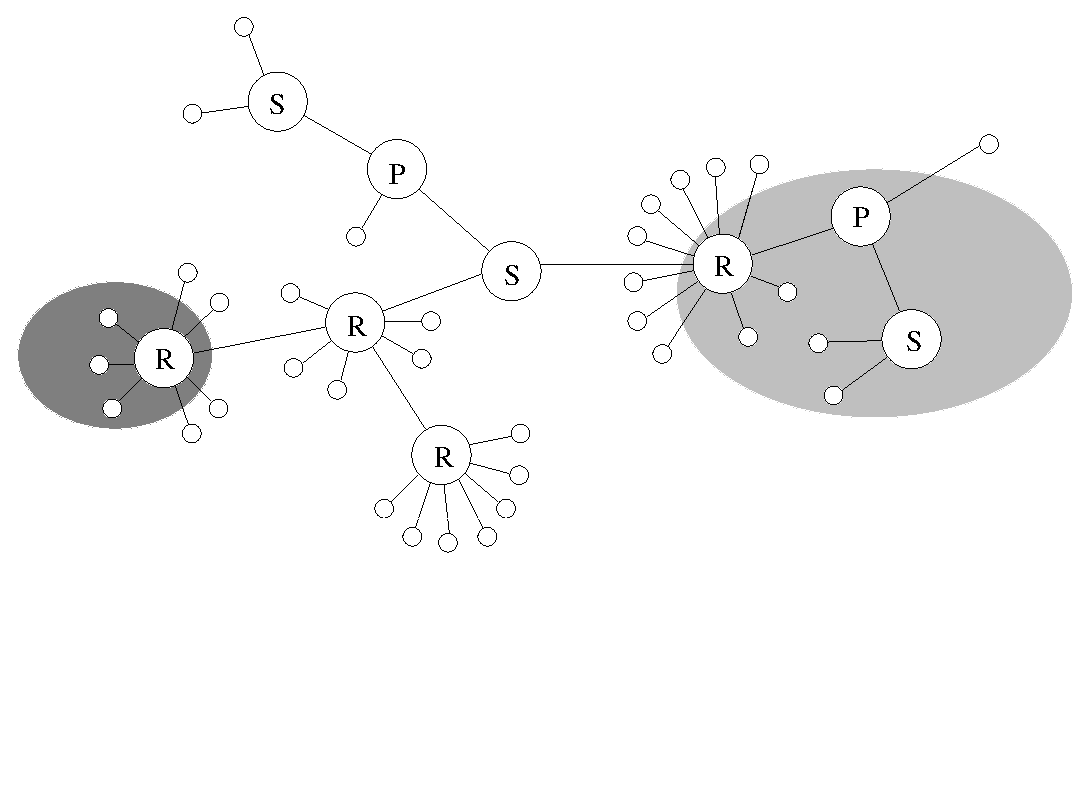
\includegraphics[width=8cm]{figure/esempio-figura-1.eps} 
\end{center}
\caption{Schema che descrive le fasi del protocollo facendo particolare attenzione al canale quantistice e canale classico.} 
\end{figure}

\subsection{Produzione, trasmissione e ricezione del segnale quantistico}\label{subse:sottosezione2-1-1}
Alice prepara gli stati coerenti andando a estrarre i valori delle componenti di quadratura \textit{q} e \textit{p} da una distribuzione normale centrata in zero ($Q\sim P\sim N (0, V_{mod})$)~\cite{https://doi.org/10.1002/qute.201800011}. Da notare che la distribuzione normale dalla quale Alice estrae le componenti di quadratura non ha nulla a che fare con le distribuzioni normali che caratterizzano gli stati coerenti ma rappresenta in modo in cui i dati vengono modulati. Dopo la preparazione Alice trasmette a Bob gli stati coerenti attraverso un canale quantistico.

Il canale \`e caratterizzato da un certo valore di trasmittanza $T$ e di rumore $\xi$. A causa della trasmittanza durante la trasmissione il segnale perde potenza quindi le gaussiane che descrivono lo stato coerente saranno centrata in un valore pi\`u vicino allo zero rispetto al momento della preparazione, mentre il rumore che viene introdotto fa aumentare la varianza delle gaussiane cos\`i da accrescere l'incertezza nelle misure da parte di Bob.

Per dare una rappresentazione matematica di quello che avviene ad uno stato coerente durante la trasmissione, possiamo andare a cosiderare un generico stato scelto da Alice $|a_i \rangle = | q_A + i p_A\rangle$. Come abbiamo detto nella sezione~\ref{se:sezione1-1} le componenti di quadratura rispondono ad una distribuzione di probabili\`a normale, quindi avremo:
\begin{equation}
\begin{split}
q_A \sim N(q_A, 1) \\
p_A \sim N(p_A, 1)
\end{split}
\end{equation}
In ricezione, a causa del canale, Bob andr\`a ad effettuare la misura su uno stato coerente alterato $|b_i \rangle = | q_B + i p_B\rangle$ dove le componenti di quadratura rispondono alle seguenti distribuzioni gaussiane:
\begin{equation}
\begin{split}
q_B \sim N(\sqrt{T} q_B, 1 + \xi) \\
p_B \sim N(\sqrt{T} p_B, 1 + \xi)
\end{split}
\end{equation}

Per la misura dello stato coerente possono essere adottati due metodi diversi:
\begin{itemize}
\item \textbf{misura omodina}: Bob decide se misurare la componente di quadratura \textit{q} o \textit{p}, la decisione viene presa attraverso una distribuzione di probabilit\`a uniforme.
\item \textbf{misura eterodina}: questa misura permette di misurare entrambe le componenti contemporaneamente, per\`o c'\`e un prezzo da pagare perch\'e effettuando questa misura viene aggiunto del rumore e la varianza delle distribuzioni normali ha un incremento di $1$.
\end{itemize}  

In caso di misura omodina \`e necessaria un'operazione addizionale cio\'e il sifting. A questo punto del protocollo Alice \`e in posseso del doppio dei dati di Bob (in quanto Bob misura solo una della due componenti per ogni round) e per far si che abbiano la stessa quantit\`a di dati correlati Bob rivela ad Alice, su canale classico publico, quale componente ha misurato ad ogni round; Alice prende nota della componenti misurate e scarta le altre.\cite{milicevic_key_2018}

\subsection{Stima dei parametri}\label{subse:stima-parametri}
Dopo avere terminato la fase di trasmissione degli stati, Alice e Bob rivelano una porzione random di dati in modo tale da confrontare ci\`o che \`e stato effetivamente inviato da Alice con le misure di Bob. Da questo confronto sono in grado di stimare l'effettiva trasmittanza e rumore in eccesso del canale di trasmissione e con queste stime possono calcolare l'informazione mutua $I_{AB}$ (informazione mutua tra Alice e Bob) e l'informazione mutua tra Eve e Bob $\chi_{EB}$. Nel caso in cui $\chi_{EB}$ risulti essere maggiore di $\beta I_{AB}$ \footnote{$\beta$ rappresenta l'accuratezza nel procesare i dati dopo la trasmissione e viene calcolata come il rapporto tra il code-rate scelto e la mutua informazione tra Alice e Bob} il protocollo viene abbortito.

\subsection{Riconciliazione delle informazioni}\label{subse:riconciliazione}
Se la stima dei parametri ha avuto successo Alice e Bob effettuano una correzione degli errori dei segnali scambiati. La riconciliazione pu\`o avvenire in due forme: 

\begin{itemize}
\item \textbf{diretta}: i dati di Alice sono i dati primari e Bob corregge i suoi dati di conseguenza.
\item \textbf{inversa}: in questo caso sono i dati di Bob ad essere primari, vengono inviati ad Alice la quale li utilizza per correggere i propri dati.
\end{itemize} 
 
La riconciliazione diretta presenta un problema: non pu\`o essere utilizzata per valori di trasmittanza troppo bassi, questo perch\'e Eve avrebbe pi\'u informazione sui dati di Alice rispetto a Bob e quindi risulter\`a impossibile creare una chiave crittografica sicura. D'altro canto la riconciliazione inversa non presenta questo problema quindi \`e possibile utilizzarla anche con valori bassi di trasmittanza, per\`o \`e da tenere in considerazione che pi\`u bassa \`e la trasmittanza pi\`u sar\`a distruttivo l'effetto del rumore del canale.\cite{https://doi.org/10.1002/qute.201800011}

A questo punto del protocollo Alice e Bob sono possesso del subset di dati non utilizzati per la stima dei parametri che andiamo a chiamare $\textbf{X}_0$ e $\textbf{Y}_0$; prima di effettuare la reconciliazione vengono prodotte, a partire dai dati in loro possesso, altre due sequenze di dati correlati. 

Quello che ci aspettiamo \`e che le varianze dei dati il possesso ad Alice e Bob siano rispettivamente:
\begin{equation}
\begin{split}
V_{X_0} &= V_{mod} + 1 \\
V_{Y_0} &= T V_{mod} + 1 + \xi
\end{split}
\end{equation}
Detto questo possiamo normalizzare $\textbf{X}_0$ e $\textbf{Y}_0$ in questo modo:
\begin{equation}
\begin{split}
\textbf{X} &= \frac{\textbf{X}_0}{\sqrt{V_{mod}}}\\
\textbf{Y} &= \frac{\textbf{Y}_0}{\sqrt{T V_{mod} + 1 + \xi}}
\end{split}
\end{equation}
Cos\`i facendo abbiamo ottenuto altre due sequenze di dati $\textbf{X}$ e $\textbf{Y}$, correlate tra loro dall'equazione $\textbf{X} = \textbf{Y} + \textbf{Z}$, dove $\textbf{Z}$ \`e una variabile aleatoria che risponde ad una distribuzione normale centrata in zero e con variaza $V_z = \frac{1}{V_{mod}}$. Quindi normalizzando in questo modo abbiamo ottenuto lo stesso effetto che avremmo avuto se Bob avesso inviato ad Alice i proprio dati normalizzati $\textbf{Y}$ su un canale che aggiunge solamente rumore gaussiano\cite{milicevic_key_2018}.

Il passo successivo per Bob sar\`a quello di generare una stringa di bit random $\underline{s} \in \{0,1\}^k$. Attraverso algoritmi di codifica LDPC viene calcolata una matrice \textbf{H} necessaria per aggiungere alla stringa \underline{s} dei bit ridondanti di parit\`a ottenendo la stringa $\underline{c} \in \{0,1\}^n$ dove $n$ corrisponde alla lunghezza della sottosequenza di dati non utilizzati per la stima dei parametri.

Successivamente \underline{c} viene utilizzata per modulare il segno della sequenza \textbf{Y} ottendo cos\`i un nuovo messaggio \underline{m} tale che $m_i = Y_i(-1)^{c_i}$ per $i = 1,2,\dots,n$.

Il messaggio \underline{m} viene trasmesso ad Alice su canale classico publico che assumiamo non introduca errori. Alice estrae da \underline{m} un messaggio fittizio \underline{r} con $r_i = \frac{m_i}{\textbf{X}_i}$ che corrisponde alla trasmisione su un canale Gaussiano con rumore di varianza $V_i = \frac{V_z}{|\textbf{X}_i|}$.

Infine ver\`a utilizzato un algoritmo LDPC di decodifica per ottenere una stima $\hat{\underline{s}}$ della stringa $\underline s$ prodotta da Bob.

\section{Discussione della sicurezza contro attacchi di lettura del segnale}
Questo protocollo \`e particolarmente sicuro perch\'e consentente il rilevamento di un eventuale spia (Eve). Nel protocollo si assume che Eve sia in possesso di un computer quantistico e che abbia accesso completo al canale di comunicazione ed anche con queste assunzioni si \`e in grado di garantire la sicurezza per diversi tipi di attacchi.

Gli attacchi presi in considerazione tipicamente sono tre e differiscono per la loro efficacia:
\begin{itemize}
\item \textbf{attacchi individuali}: Eve effettua operazioni singolarmente su ogni segnale che viene scambiato tra Alice e Bob. 
\begin{figure}[tbp] 
\begin{center}
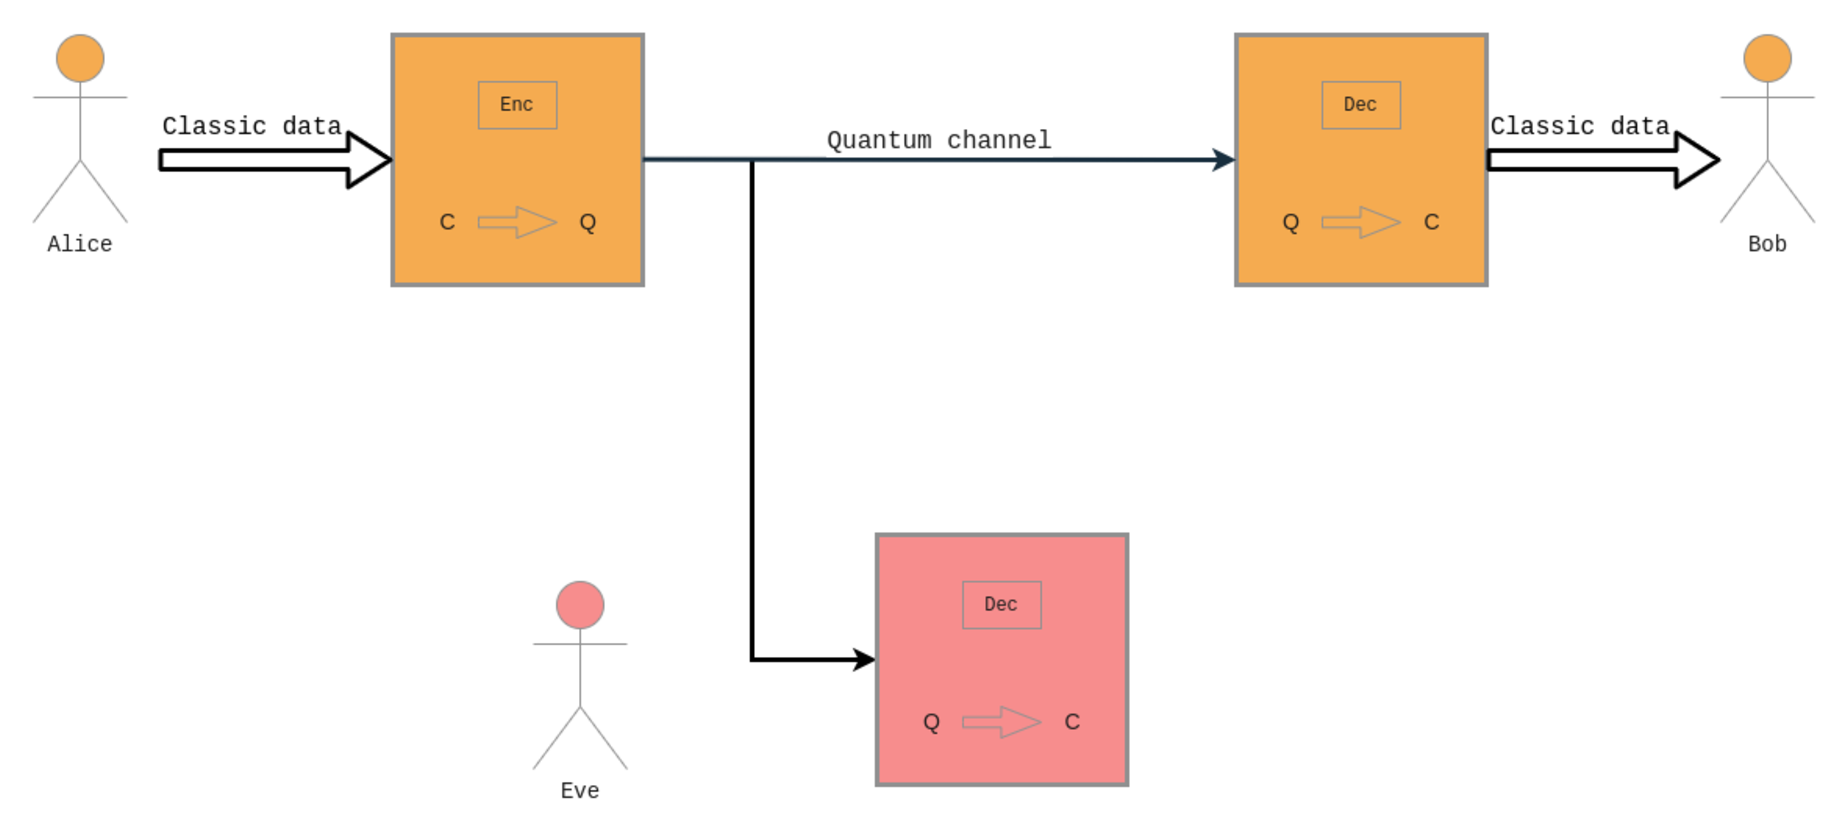
\includegraphics[width=0.8\textwidth]{figure/individual_attack.eps} 
\end{center}
\caption{Schema di comunicazione tra Alice e Bob Sezione~\ref{se:prima-sezione}.} \label{fig:figura-doppia}
\end{figure}
\item \textbf{attacchi collettivi}: Eve salva nella memoria del suo computer quantistico un certo numero di stati sui quali effettua una misura collettiva. Questo attacco \`e pi\`u potente del precedente perch\`e secondo i pricipi della fisica quantistica effettuando una misura collettiva si pu\`o potenzialmente ricavare pi\`u informazione che dalla misura del singolo stato.
\begin{figure}[tbp] 
\begin{center}
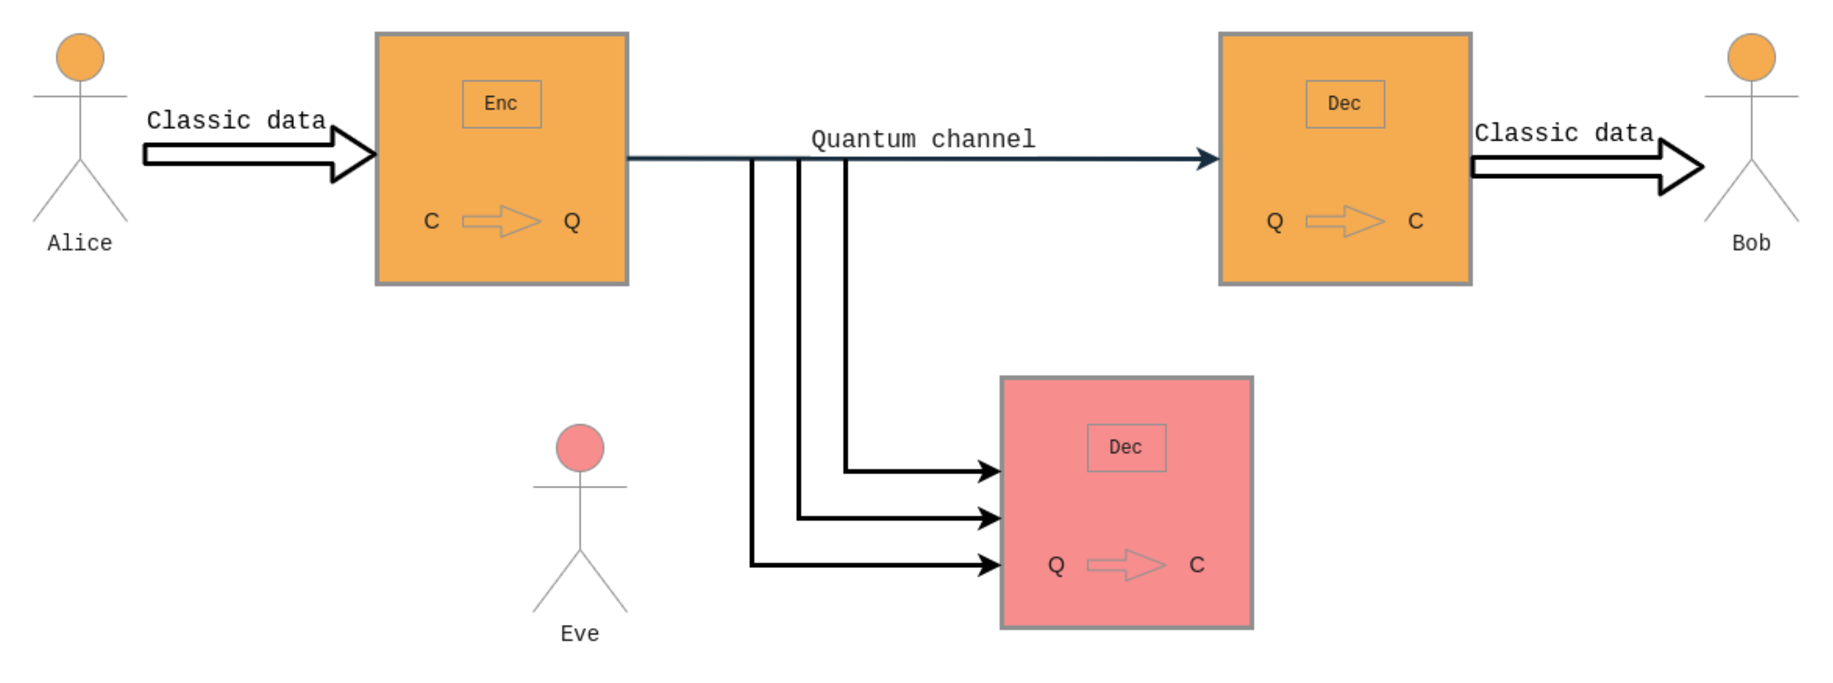
\includegraphics[width=0.8\textwidth]{figure/collective_attack.eps} 
\end{center}
\caption{Schema di comunicazione tra Alice e Bob Sezione~\ref{se:prima-sezione}.} \label{fig:figura-doppia}
\end{figure}
\item \textbf{attacchi coerenti}: sono attacchi pi\`u potenti dei collettivi perché Eve, oltre alla lettura collettiva, può utilizzare delle correlazioni quantistiche, cioé entanglement, per mettere in relazione gli stati di pi\`u run.
\begin{figure}[tbp] 
\begin{center}
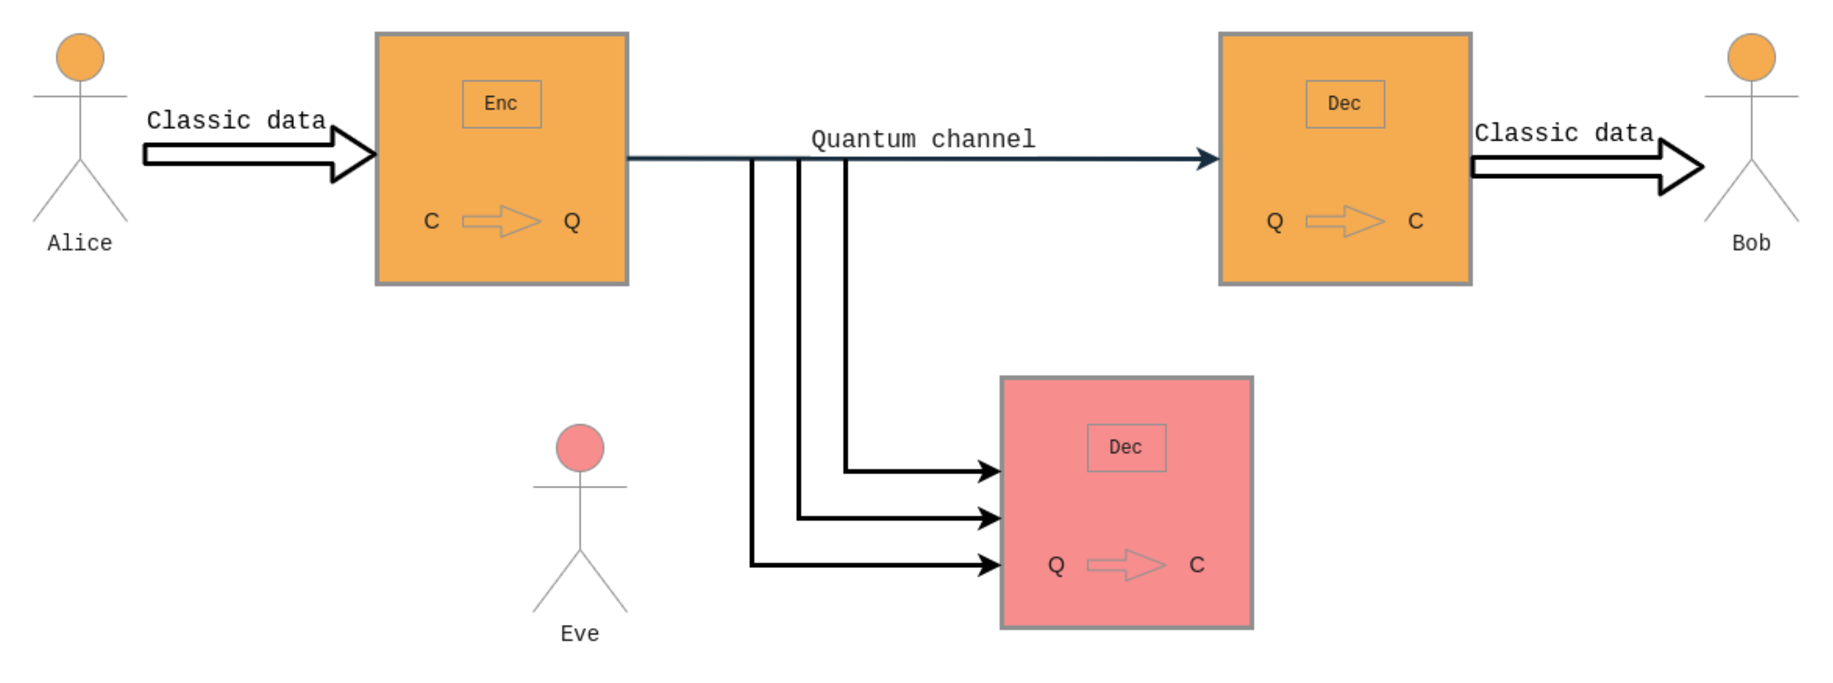
\includegraphics[width=0.8\textwidth]{figure/collective_attack.eps} 
\end{center}
\caption{Schema di comunicazione tra Alice e Bob Sezione~\ref{se:prima-sezione}.} \label{fig:figura-doppia}
\end{figure}
\end{itemize} 

Tornando al motivo per cui effettivamente si riesce a rilevare Eve possiamo, anche questa volta, dare il merito ai principi della fisica quantistica. Questo perch\`e in caso di misura da parte di Eve lo stato coerente trasmesso verr\`a alterato. Due esempio di attacchi che Eve pu\`o mettere in atto e le loro conseguenze sono: 
\begin{itemize}
\item sottrarre una parte del segnale per effettuare una misura sullo stesso, questo comporta una diminuzione di fotoni del segnale ricevuto da Bob
\item misura il segnale attraverso una misura eterodina per stimare entrambe le componenti di quadratura. Utilizzando le componenti misurate come valori medi, realizza un nuovo stato coerente che trasmette a Bob. In questo modo siccome vengono misurati dei valori randomici e siccome la misura eterodina stessa introduce ulteriore rumore la varianza degli stati coerenti ricevuti da Bob sar\`a superiore a quella originaria. 
\end{itemize} 
In entrambi i casi, un attacco da parte di Eve non va a far altro che aumentare gli effetti distruttivi del canale di trasmissione.


Tutte queste alterazione, in fase di stima dei parametri, produrranno dei valori indesiderati come $\chi > I_{AB}$. Queste incongruenza tra le stime e ci\`o che ci si aspettava dalla scelta dei paramettri iniziali portano a pensare che una spia si sia intromessa nella comunicazione. 

\begin{figure}[h] 
\begin{center}
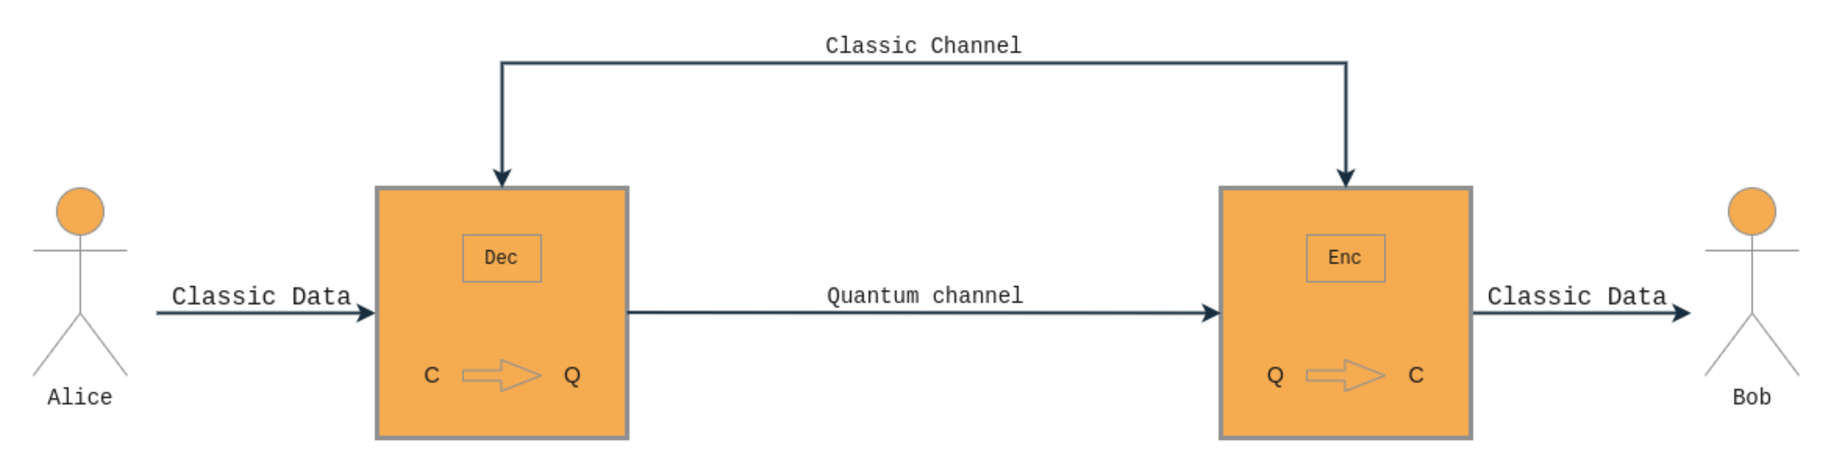
\includegraphics[width=\textwidth]{figure/alice_bob_communication.eps} 
\end{center}
\caption{Schema di comunicazione tra Alice e Bob Sezione~\ref{se:prima-sezione}.} \label{fig:figura-doppia}
\end{figure}

